% =====================================================================
%  MedGuardAI -- Project Documentation
%  Compile with:  pdflatex MedGuardAI.tex   (run twice for the ToC/refs)
% =====================================================================
\documentclass[11pt,a4paper]{article}

\usepackage[T1]{fontenc}
\usepackage[utf8]{inputenc}
\usepackage{lmodern}
\usepackage{amsmath}
\usepackage[margin=2.3cm]{geometry}
\usepackage{graphicx}
\usepackage{float}
\usepackage{xcolor}
\usepackage{tikz}
\usepackage{pgfplots}
\pgfplotsset{compat=1.18}
\usetikzlibrary{positioning,arrows.meta,shapes.geometric,calc,fit,backgrounds}
\usepackage{booktabs}
\usepackage{array}
\usepackage{tabularx}
\usepackage{enumitem}
\usepackage{titlesec}
\usepackage{caption}
\usepackage{fancyhdr}
\usepackage[hidelinks]{hyperref}

% ---------------------------------------------------------------- palette
\definecolor{medink}{HTML}{1F2937}
\definecolor{medblue}{HTML}{15616D}
\definecolor{medaccent}{HTML}{2A9D8F}
\definecolor{medslate}{HTML}{7D8597}
\definecolor{medsand}{HTML}{E07A3F}
\definecolor{medred}{HTML}{C44536}
\definecolor{medbg}{HTML}{F1F5F9}

\hypersetup{colorlinks=true,linkcolor=medblue,urlcolor=medblue,citecolor=medblue}

% ---------------------------------------------------------------- headings
\titleformat{\section}{\Large\bfseries\color{medblue}}{\thesection.}{0.5em}{}[{\color{medaccent!55}\titlerule[1.2pt]}]
\titlespacing*{\section}{0pt}{1.5em}{0.6em}
\titleformat{\subsection}{\large\bfseries\color{medink}}{\thesubsection}{0.5em}{}
\titlespacing*{\subsection}{0pt}{1.0em}{0.35em}

\captionsetup{font=small,labelfont={bf,color=medblue},labelsep=period}

% ---------------------------------------------------------------- header/footer
\pagestyle{fancy}
\fancyhf{}
\renewcommand{\headrulewidth}{0.4pt}
\fancyhead[L]{\small\color{medslate}MedGuardAI Project Documentation}
\fancyhead[R]{\small\color{medslate}\thepage}

% ---------------------------------------------------------------- callout box
\newcommand{\callout}[2]{%
\par\vspace{6pt}\noindent
\begin{tikzpicture}
\node[draw=medaccent,line width=1pt,fill=medaccent!8,rounded corners=4pt,
      inner sep=10pt,text width=\dimexpr\linewidth-24pt\relax,align=left] (cb)
{{\bfseries\color{medblue}#1}\par\vspace{3pt}#2};
\end{tikzpicture}\par\vspace{6pt}}

% ---------------------------------------------------------------- tikz styles
\tikzset{
  box/.style   ={rounded corners=3pt,draw=medblue!75,fill=medblue!8,line width=0.8pt,align=center,inner sep=6pt,font=\small,minimum height=10mm},
  stage/.style ={box,fill=medaccent!16,draw=medaccent!80},
  guard/.style ={box,fill=medred!10,draw=medred!65},
  data/.style  ={draw=medslate!85,fill=medslate!12,line width=0.7pt,align=center,inner sep=6pt,font=\footnotesize\itshape,rounded corners=1pt},
  store/.style ={box,fill=medslate!18,draw=medslate!85,font=\footnotesize},
  dec/.style   ={diamond,aspect=2.2,draw=medblue!75,fill=medblue!8,line width=0.8pt,align=center,font=\footnotesize,inner sep=0pt},
  term/.style  ={rounded corners=8pt,draw=medink,fill=medink!10,line width=0.8pt,font=\small\bfseries,align=center,inner sep=6pt},
  arr/.style   ={-{Stealth[length=2.4mm]},line width=0.8pt,draw=medink!85},
  darr/.style  ={arr,dashed},
  lbl/.style   ={font=\footnotesize\itshape,fill=white,inner sep=1.5pt},
}

% =====================================================================
\begin{document}

% ---------------------------------------------------------------- title page
\thispagestyle{empty}
\vspace*{1.2cm}
\begin{center}
{\color{medaccent}\rule{\linewidth}{2pt}}\\[10pt]
{\Huge\bfseries\color{medblue}MedGuardAI}\\[10pt]
{\large\itshape Safety-First Medical Assistant powered by Agentic RAG}\\[5pt]
{\large Project Documentation}\\[10pt]
{\color{medaccent}\rule{\linewidth}{2pt}}\\[24pt]
{\large
Borodi Bogdan-Vasile \;\textbullet\; Moca Andrei-Catalin \;\textbullet\; Petrea Alexandra\\[3pt]
Pauliuc C\u{a}lin George \;\textbullet\; Vaicum Ana Maria}\\[22pt]
{\normalsize
\textbf{Course:} Large Language Models, Faculty of Mathematics and Computer Science\\[4pt]
\textbf{Repository:} \url{https://github.com/andreimoca/MedGuardAI} \qquad \textbf{Date:} May 2026}
\end{center}

\vspace{18pt}
\callout{In one line}{Ask a medical question together with a short patient profile (age, weight,
allergies, conditions); get back a brief, FDA-grounded answer, an automatic hand-off to emergency
care when warranted, and a thumbs-up / thumbs-down control whose corrections feed the model's next
training round.}

\vspace{6pt}
\callout{Headline result}{Fine-tuning the model (QLoRA supervised fine-tune + a DPO / RLHF pass)
raises the rule-based pass rate on a held-out evaluation set from \textbf{67.9\%} to \textbf{89.6\%},
with the biggest gains on the safety-critical categories: hallucination handling
(0\%\,$\to$\,77.8\%) and drug Q\&A (+15.6 pp).}

\vfill
{\small\color{medslate}Research prototype. Not a substitute for professional medical advice.}
\clearpage

% ---------------------------------------------------------------- ToC
\tableofcontents
\clearpage

% =====================================================================
\section{Overview}

MedGuardAI answers everyday questions about medications and symptoms. Its first priority is not
correctness for its own sake but \emph{safety}: every answer is grounded in official FDA drug labels,
the model is instructed to decline rather than guess, and a layered guard system catches unsafe or
hallucinated output before the user ever sees it. The whole system runs locally, so medical data
never leaves the machine.

It is built as an \textbf{agent}. For each query, a small state machine (LangGraph) decides which of
six clinical tools to call (drug-information lookup, dosage calculation, drug-interaction
check, allergy check, emergency triage, and a live FDA fallback), always grounded by
retrieval over a local vector database of drug leaflets, and always personalised with the patient's
age, weight, allergies and conditions.

The reasoning model is a \textbf{fine-tuned Small Language Model}: a QLoRA supervised fine-tune of
Google Gemma-3-4b, followed by a DPO (Direct Preference Optimization) pass that uses real user
feedback. Against the course rubric this targets the ``fine-tuned SLM'' tier, and the corresponding
requirements are all in place:

\begin{itemize}[leftmargin=1.4em,itemsep=2pt,topsep=3pt]
  \item \textbf{Data ingestion} of new datasets: an OpenFDA / DailyMed label pipeline plus MedQuAD (via Kaggle) for fine-tuning;
  \item \textbf{RAG}: ChromaDB vector store, sentence-transformer embeddings, MMR retrieval;
  \item \textbf{Agent architecture}: a LangGraph graph wired to six clinical tools;
  \item \textbf{Task-specific fine-tuning}: QLoRA SFT on a curated medical Q\&A and triage set;
  \item \textbf{RLHF}: DPO on preference data, including a live human-feedback loop;
  \item \textbf{Toxicity / hallucination handling}: input and output guards plus a groundedness check;
  \item \textbf{Evaluation}: a hand-curated held-out test set with a base-vs-fine-tuned comparison.
\end{itemize}

% =====================================================================
\section{System Architecture}

\begin{figure}[H]
\centering
\resizebox{\textwidth}{!}{%
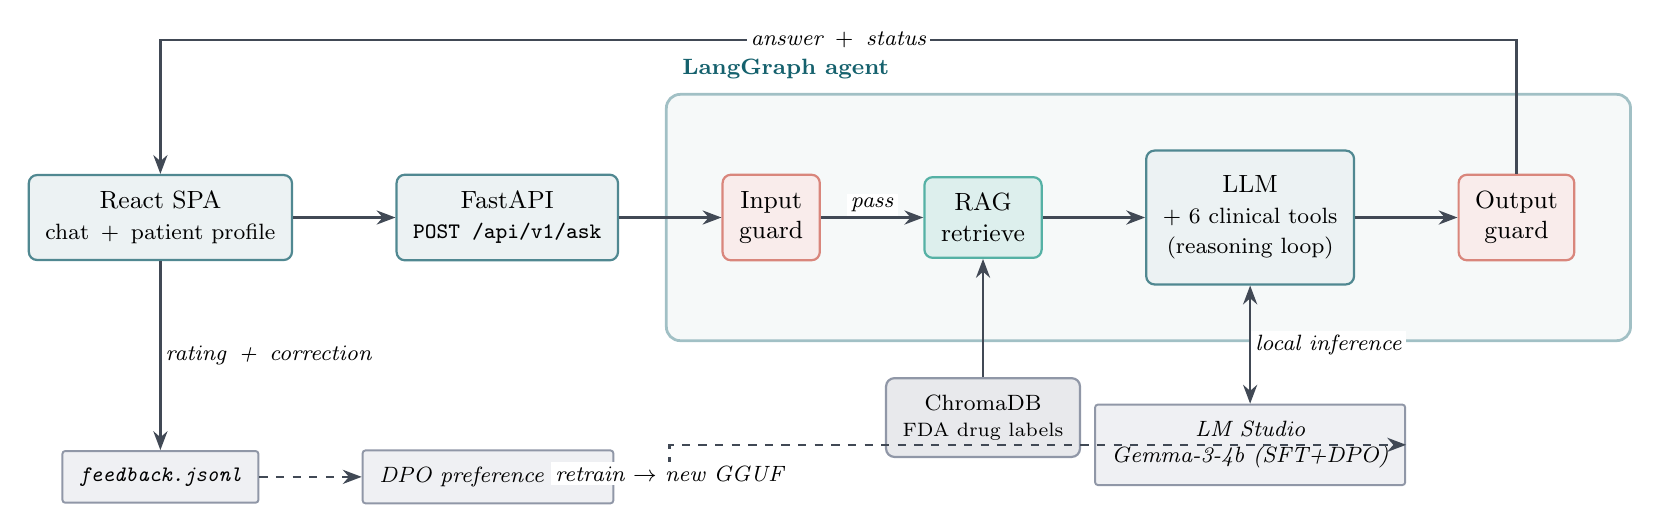
\begin{tikzpicture}[node distance=11mm and 13mm]
  \node[box] (ui) {React SPA\\{\footnotesize chat \,+\, patient profile}};
  \node[box, right=of ui] (api) {FastAPI\\{\footnotesize \texttt{POST /api/v1/ask}}};
  \node[guard, right=of api] (ig) {Input\\guard};
  \node[stage, right=of ig] (rt) {RAG\\retrieve};
  \node[box, right=of rt, minimum height=17mm] (ag) {LLM\\{\footnotesize + 6 clinical tools}\\{\footnotesize (reasoning loop)}};
  \node[guard, right=of ag] (og) {Output\\guard};

  \node[store, below=15mm of rt] (chr) {ChromaDB\\{\scriptsize FDA drug labels}};
  \node[data,  below=15mm of ag] (lms) {LM Studio\\Gemma-3-4b (SFT+DPO)};
  \node[data,  below=24mm of ui] (fb)  {\texttt{feedback.jsonl}};
  \node[data,  right=of fb]       (dpo) {DPO preference data};

  \draw[arr] (ui) -- (api);
  \draw[arr] (api) -- (ig);
  \draw[arr] (ig) -- node[lbl,above]{pass} (rt);
  \draw[arr] (rt) -- (ag);
  \draw[arr] (ag) -- (og);
  \draw[arr] (chr) -- (rt);
  \draw[{Stealth[length=2.4mm]}-{Stealth[length=2.4mm]},line width=0.8pt,draw=medink!85] (lms) -- node[lbl,right]{local inference} (ag);
  % return path
  \coordinate (rmid) at ($(og.north)!0.5!(ui.north)$);
  \draw[arr] (og.north) -- ++(0,17mm) coordinate (rtop) -| (ui.north);
  \node[lbl] at (rmid |- rtop) {answer \,$+$\, status};
  % feedback loop
  \draw[arr]  (ui.south) -- node[lbl,right]{rating \,+\, correction} (fb.north);
  \draw[darr] (fb) -- (dpo);
  \draw[darr] (dpo.east) -- ++(7mm,0) |- node[lbl,pos=0.25,below]{retrain $\rightarrow$ new GGUF} (lms.east);

  \begin{scope}[on background layer]
    \node[draw=medblue!40,line width=1pt,rounded corners=5pt,fill=medblue!4,
          fit=(ig)(rt)(ag)(og),inner sep=7mm] (agentbox) {};
  \end{scope}
  \node[anchor=south west, font=\footnotesize\bfseries, text=medblue]
        at ([yshift=0.6mm]agentbox.north west) {\;LangGraph agent};
\end{tikzpicture}}
\caption{End-to-end request flow. The browser sends a question and the patient profile to FastAPI;
the LangGraph agent screens the input, retrieves drug-label context, reasons with the local Gemma
model and its tools, and the output guard fact-checks the answer before it returns. Ratings and
corrections collected in the UI become preference data for the next DPO round.}
\end{figure}

\noindent\textbf{Request lifecycle.} A query from the React SPA (carrying the patient profile) hits
\texttt{POST /api/v1/ask}. A fast keyword check short-circuits obvious emergencies; otherwise the
request enters the LangGraph agent. The input guard screens it, retrieval pulls the most relevant
drug-label passages, the model answers (calling clinical tools as needed)
and the output guard sanitises the text, checks it against the retrieved context, and appends source
labels. The answer (with a \texttt{success} or \texttt{emergency} status) returns to the UI, where the
user can rate it; ratings and corrections are appended to \texttt{feedback.jsonl}, the raw material
for the next preference-tuning round.

\begin{table}[H]
\centering
\renewcommand{\arraystretch}{1.25}
\caption{Components and the role each one plays.}
\begin{tabular}{@{}>{\bfseries\raggedright\arraybackslash}p{0.155\textwidth}
                   >{\raggedright\arraybackslash}p{0.335\textwidth}
                   >{\raggedright\arraybackslash}p{0.44\textwidth}@{}}
\toprule
\normalfont\bfseries Layer & \normalfont\bfseries Technology & \normalfont\bfseries Role\\
\midrule
Frontend & React 18 + Vite + Framer Motion & Chat UI, patient-profile sidebar, thumbs-up / thumbs-down feedback controls.\\[3pt]
API & FastAPI (async Python) & Endpoints \texttt{/api/v1/ask}, \texttt{/api/v1/feedback}, \texttt{/health}.\\[3pt]
Agent layer & LangGraph & State machine wiring the guards, retrieval, the model and its tools.\\[3pt]
Retrieval & ChromaDB + Sentence-Transformers (\texttt{all-MiniLM-L6-v2}) & Semantic search over FDA drug labels (persistent vector store).\\[3pt]
Inference & Google Gemma-3-4b (QLoRA SFT + DPO), served by LM Studio & The reasoning model, run locally over an OpenAI-compatible endpoint.\\[3pt]
Safety & Detoxify + rule guards + embedding-based groundedness & Input / output screening, hallucination and toxicity checks.\\[3pt]
Data & OpenFDA / DailyMed labels; MedQuAD (Kaggle) & Knowledge base for RAG; medical Q\&A corpus for fine-tuning.\\
\bottomrule
\end{tabular}
\end{table}

% =====================================================================
\section{Agent Architecture and Tools}

The agent is a compiled LangGraph graph (Figure~\ref{fig:graph}). Control starts at the input guard;
a blocked query returns a refusal immediately, without ever invoking the model. Otherwise retrieval
always runs first, so the model never answers without context. The model may then loop through tool
calls (each tool result is fed back into the conversation) until it produces
a final answer, which the output guard post-processes before the graph ends. The patient profile is
injected into every model turn, so dosage, allergy and triage reasoning is personalised rather than
generic.

\begin{figure}[H]
\centering
\resizebox{\textwidth}{!}{%
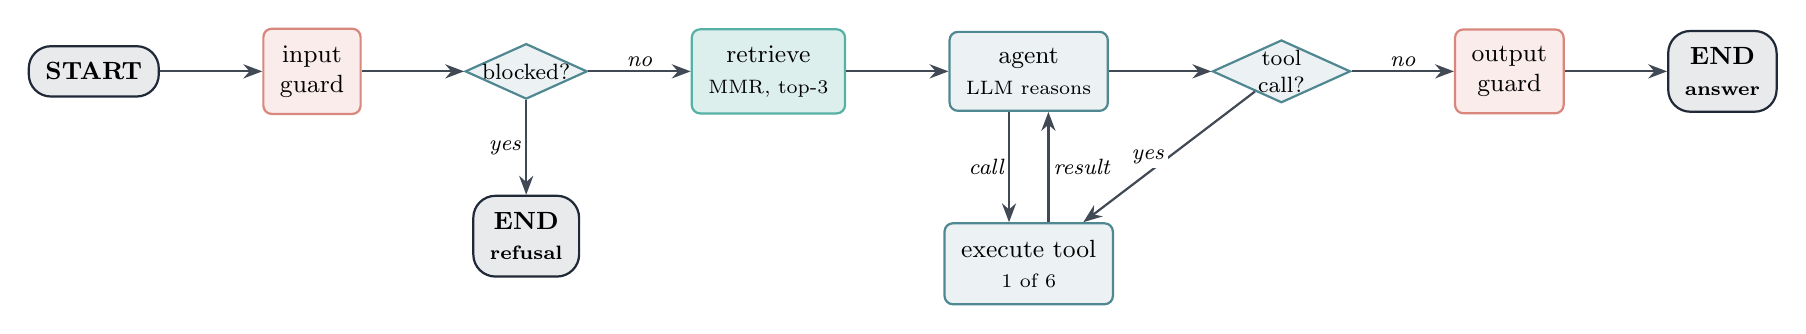
\begin{tikzpicture}[node distance=9mm and 13mm]
  \node[term] (start) {START};
  \node[guard, right=of start] (ig) {input\\guard};
  \node[dec,  right=of ig]    (d1) {blocked?};
  \node[stage,right=of d1]    (rt) {retrieve\\{\scriptsize MMR, top-3}};
  \node[box,  right=of rt]    (ag) {agent\\{\scriptsize LLM reasons}};
  \node[dec,  right=of ag]    (d2) {tool\\call?};
  \node[guard,right=of d2]    (og) {output\\guard};
  \node[term, right=of og]    (end) {END\\{\scriptsize answer}};

  \node[term, below=12mm of d1] (endr)  {END\\{\scriptsize refusal}};
  \node[box,  below=14mm of ag] (tools) {execute tool\\{\scriptsize 1 of 6}};

  \draw[arr] (start) -- (ig);
  \draw[arr] (ig) -- (d1);
  \draw[arr] (d1) -- node[lbl,left]{yes} (endr);
  \draw[arr] (d1) -- node[lbl,above]{no} (rt);
  \draw[arr] (rt) -- (ag);
  \draw[arr] (ag) -- (d2);
  \draw[arr] (d2) -- node[lbl,left]{yes} (tools);
  \draw[arr] ([xshift=-2.5mm]ag.south) -- node[lbl,left]{call} ([xshift=-2.5mm]tools.north);
  \draw[arr] ([xshift= 2.5mm]tools.north) -- node[lbl,right]{result} ([xshift= 2.5mm]ag.south);
  \draw[arr] (d2) -- node[lbl,above]{no} (og);
  \draw[arr] (og) -- (end);
\end{tikzpicture}}
\caption{The LangGraph state machine. Retrieval runs before the model on every accepted query; the
model loops through tool calls until it is ready to answer; the output guard always runs last.}
\label{fig:graph}
\end{figure}

\begin{table}[H]
\centering
\renewcommand{\arraystretch}{1.25}
\caption{The six clinical tools the agent can call.}
\begin{tabular}{@{}>{\ttfamily\footnotesize\raggedright\arraybackslash}p{0.235\textwidth}
                   >{\footnotesize\raggedright\arraybackslash}p{0.155\textwidth}
                   >{\raggedright\arraybackslash}p{0.53\textwidth}@{}}
\toprule
\normalfont\bfseries Tool & \normalfont\bfseries Inputs & \normalfont\bfseries What it does\\
\midrule
retrieve\_drug\_info & query & Semantic search over the FDA-label vector store; returns the top passages with their drug names.\\[3pt]
dosage\_calculator & drug, age, weight & Returns the FDA dosage section plus pediatric / geriatric / low-body-weight flags for this patient.\\[3pt]
check\_drug\_interactions & drug A, drug B & Scans drug A's label for documented interactions with drug B.\\[3pt]
check\_allergies & drug, patient allergies & Cross-references the drug's active ingredients against the patient's allergies, including cross-reactivity classes (e.g.\ the penicillin family, NSAIDs).\\[3pt]
emergency\_classifier & query & Tiered pattern match (\textsc{high} / \textsc{medium} / \textsc{none}) for life-threatening presentations.\\[3pt]
fetch\_openfda\_live & drug name & Live OpenFDA lookup for drugs not in the local store; returns a condensed label.\\
\bottomrule
\end{tabular}
\end{table}

% =====================================================================
\section{Data Ingestion and RAG}

New datasets enter through the ingestion pipeline. Drug labels are fetched from the OpenFDA / DailyMed
API, split with a recursive character splitter (1000-character chunks, 200-character overlap, using a
hierarchical separator order: paragraph, then sentence, then word), embedded with
\texttt{all-MiniLM-L6-v2} (384 dimensions) and stored in a persistent ChromaDB collection.

At query time, retrieval uses MMR (Maximal Marginal Relevance): the top $k=3$ passages are selected
from a pool of $12$ candidates with $\lambda=0.7$, so the context is both relevant and
non-redundant. It runs once up front, before the model sees the question, and again on demand whenever
the model calls \texttt{retrieve\_drug\_info}. Retrieved passages are injected into the system prompt
tagged \texttt{[Source N: <drug>]}, and the prompt makes that retrieved context the primary source of
truth: the model is told to prefer it over its own parametric knowledge and to say so when
the context does not cover the question.

% =====================================================================
\section{Fine-Tuning and RLHF}

The runtime model is not stock Gemma-3-4b. It is produced in two phases on a free Colab / Kaggle T4
GPU, then exported as a quantised GGUF and served by LM Studio (Figure~\ref{fig:train}).

\begin{figure}[H]
\centering
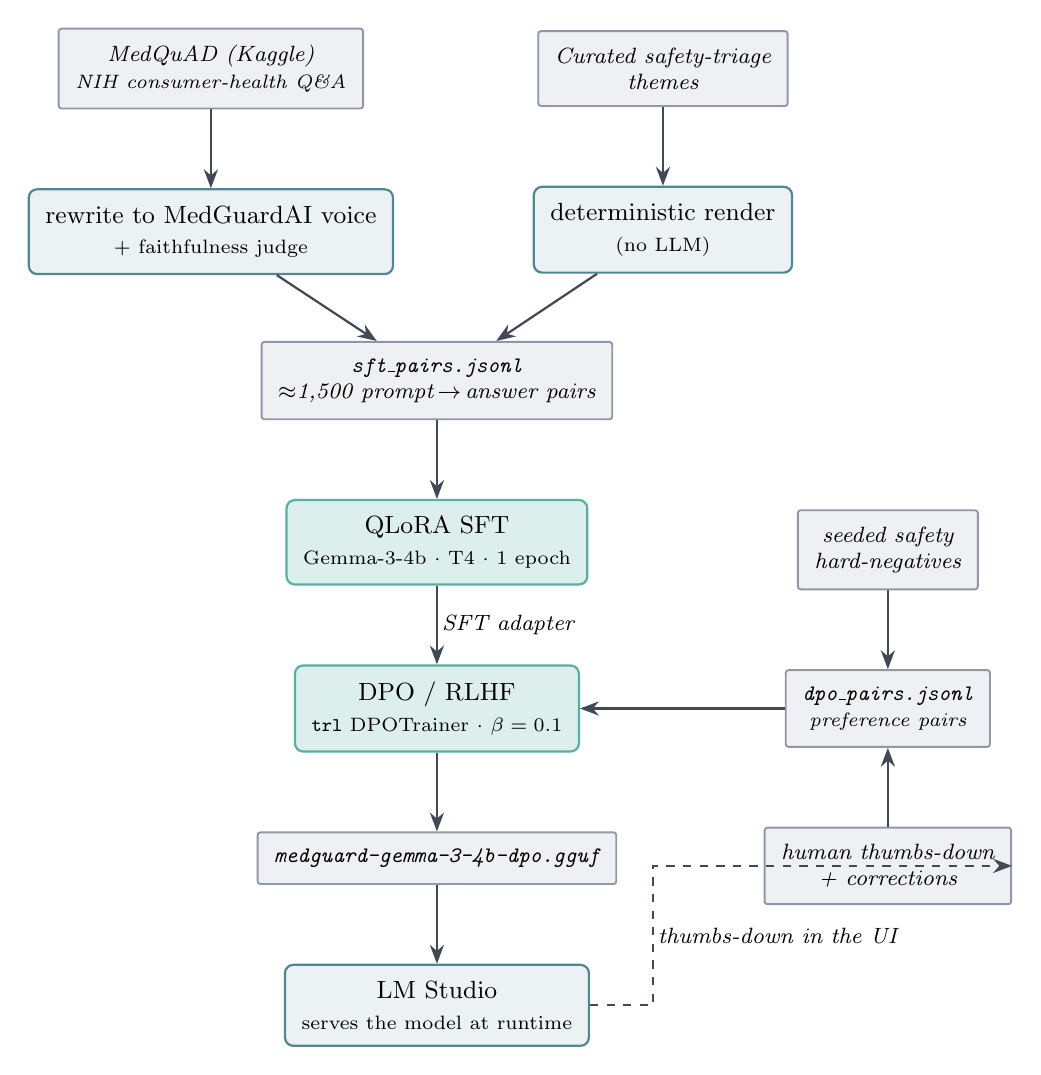
\begin{tikzpicture}[node distance=10mm and 14mm]
  \node[data] (mq)   {MedQuAD (Kaggle)\\{\scriptsize NIH consumer-health Q\&A}};
  \node[data, right=22mm of mq] (th) {Curated safety-triage\\themes};

  \node[box, below=of mq] (rw)  {rewrite to MedGuardAI voice\\{\scriptsize + faithfulness judge}};
  \node[box, below=of th] (tp)  {deterministic render\\{\scriptsize (no LLM)}};

  \coordinate (rtmid) at ($(rw)!0.5!(tp)$);
  \node[data, below=14mm of rtmid] (sft) {\texttt{sft\_pairs.jsonl}\\$\approx$1{,}500 prompt\,$\rightarrow$\,answer pairs};
  \node[stage, below=of sft] (qlora) {QLoRA SFT\\{\scriptsize Gemma-3-4b $\cdot$ T4 $\cdot$ 1 epoch}};
  \node[stage, below=of qlora] (dpo) {DPO / RLHF\\{\scriptsize \texttt{trl} DPOTrainer $\cdot$ $\beta=0.1$}};
  \node[data, below=of dpo] (gguf) {\texttt{medguard-gemma-3-4b-dpo.gguf}};
  \node[box, below=of gguf] (lms) {LM Studio\\{\scriptsize serves the model at runtime}};

  \node[data, right=26mm of dpo] (dp) {\texttt{dpo\_pairs.jsonl}\\{\scriptsize preference pairs}};
  \node[data, above=10mm of dp] (hn) {seeded safety\\hard-negatives};
  \node[data, below=10mm of dp] (hf) {human thumbs-down\\+ corrections};

  \draw[arr] (mq) -- (rw);
  \draw[arr] (th) -- (tp);
  \draw[arr] (rw) -- (sft);
  \draw[arr] (tp) -- (sft);
  \draw[arr] (sft) -- (qlora);
  \draw[arr] (qlora) -- node[lbl,right]{SFT adapter} (dpo);
  \draw[arr] (dpo) -- (gguf);
  \draw[arr] (gguf) -- (lms);
  \draw[arr] (hn) -- (dp);
  \draw[arr] (hf) -- (dp);
  \draw[arr] (dp) -- (dpo);
  \draw[darr] (lms.east) -- ++(8mm,0) |- node[lbl,pos=0.25,right]{thumbs-down in the UI} (hf.east);
\end{tikzpicture}
\caption{The training pipeline. Two phases: a supervised fine-tune on a curated medical Q\&A and
triage set, then a DPO pass on preference pairs. The dashed arrow is the human-feedback flywheel: real downvotes in the UI become preference data for the next DPO round.}
\label{fig:train}
\end{figure}

\subsection{Phase 2: Supervised fine-tuning}
The SFT set is roughly \textbf{1{,}500 prompt\,$\rightarrow$\,answer pairs}: about 1{,}360 items from
MedQuAD (a consumer-health Q\&A corpus curated from U.S.\ NIH websites, pulled via Kaggle), each
rewritten into MedGuardAI's brief, safety-first voice and kept only if a faithfulness judge confirms
the rewrite introduces no clinical fact absent from the original answer; plus about 140 symptom-triage
rows rendered from deterministic templates (no LLM) covering the low / medium / emergency tiers.

Roughly 1{,}500 tightly curated, on-task examples is a deliberate choice for a 4B model. It is large
enough to durably shift tone, formatting and safety behaviour in a single epoch on a free T4, and
small enough to remain hand-checkable and to avoid overfitting or catastrophic forgetting of the base
model's general competence. Training is QLoRA (4-bit base; LoRA $r=16$, $\alpha=16$, dropout $0.05$;
learning rate $2\times10^{-4}$ with a cosine schedule; 1 epoch; batch size 2 with gradient
accumulation 4; max sequence length 2048; \texttt{adamw\_8bit}). The merged model is exported as a
\texttt{Q4\_K\_M} GGUF.

\subsection{Phase 3: DPO (RLHF)}
Starting from the SFT adapter, a Direct Preference Optimization pass teaches the model to prefer the
safe answer over a plausible near-miss. Preference pairs come from two real, reproducible sources (no LLM is used to generate them):

\begin{itemize}[leftmargin=1.4em,itemsep=2pt,topsep=3pt]
  \item \textbf{Seeded safety hard-negatives:} deterministic \emph{(chosen, rejected)} pairs templated
        from the symptom themes, where the rejected answer breaks exactly one safety rule:
        it drops the \texttt{[EMERGENCY]} hand-off on a true emergency, over-triages a routine symptom,
        invents an overconfident dose, or names a prescription-only drug.
  \item \textbf{Human feedback:} thumbs-down events from the live UI that came with a user correction
        become \emph{(rejected = the downvoted answer, chosen = the correction)}, weighted up so the
        real signal counts for more.
\end{itemize}

Training uses \texttt{trl}'s \texttt{DPOTrainer} (learning rate $5\times10^{-6}$, $\beta=0.1$, 1
epoch). The result is exported to LM Studio; pointing the backend at the new GGUF needs no code
change. This closes the human-feedback flywheel: real usage produces corrections, corrections become
preference data, and preference data produces a safer model.

\callout{Why DPO rather than classic RLHF / PPO}{DPO optimises the same human-preference objective
without training a separate reward model or running on-policy rollouts, so it fits a free-tier GPU and
a small preference set, while $\beta=0.1$ keeps the policy anchored to the supervised
model so it does not drift.}

% =====================================================================
\section{Safety: Toxicity and Hallucination}

Two guards bracket the model (Figure~\ref{fig:safety}).

\textbf{Input guard} (before the model). Blocks prompt-injection attempts (``ignore previous
instructions'', jailbreak patterns), disallowed content (drug synthesis, weapons, recreational
misuse) and toxic language (Detoxify when available, regular expressions otherwise), returning a
polite refusal without ever invoking the model.

\textbf{Output guard} (after the model). Strips machinery that leaked into the text (stray
\texttt{[/EMERGENCY]} tags, ``based on the retrieved context\dots'' preambles, self-referential
sentences); re-checks toxicity; runs a \textbf{groundedness check}: factual claims (drug
names, dosages, contraindications) are embedded and compared against the retrieved context, so a
severely ungrounded answer is rewritten and a mildly ungrounded one gets a low-confidence note; and
appends a \texttt{Sources:}\ line listing the drug labels it relied on.

\textbf{Emergency short-circuit.} A \textsc{high}-tier presentation (crushing chest pain,
stroke signs, severe trouble breathing, suspected overdose, anaphylaxis, suicidal intent, uncontrolled
bleeding, a first seizure, fever in an infant under three months, a severe head injury) is
answered \emph{only} with an \texttt{[EMERGENCY]} hand-off, never with medication advice. The model is
told to trigger it on the user's own words, not on a warning it happened to read in a label (a side
effect listed in an FDA leaflet is not the user's current condition).

\begin{figure}[H]
\centering
\resizebox{0.95\textwidth}{!}{%
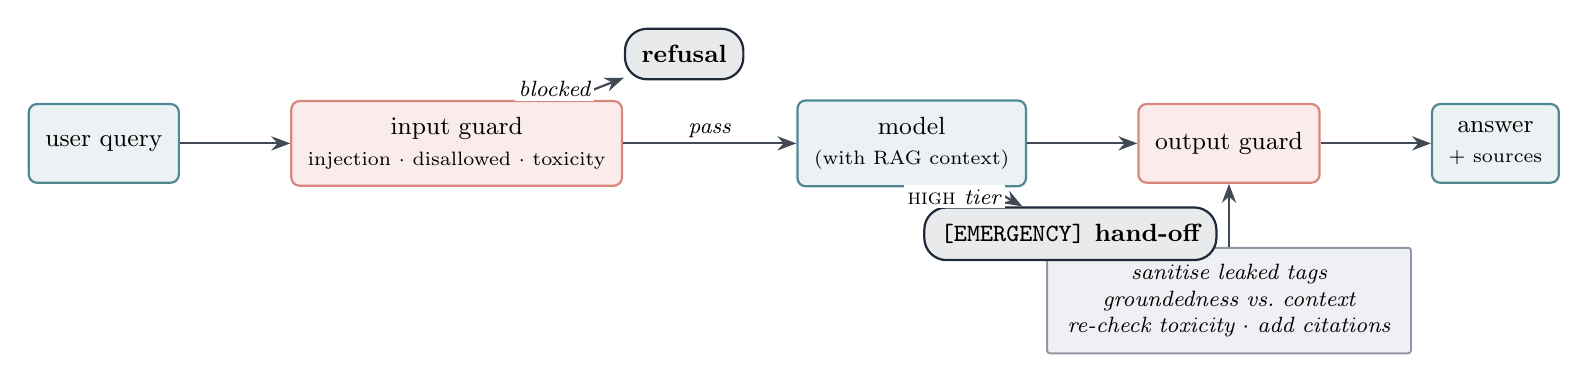
\begin{tikzpicture}[node distance=7mm and 14mm]
  \node[box] (q) {user query};
  \node[guard, right=of q] (ig) {input guard\\{\scriptsize injection $\cdot$ disallowed $\cdot$ toxicity}};
  \node[box, right=22mm of ig] (model) {model\\{\scriptsize (with RAG context)}};
  \node[guard, right=of model] (og) {output guard};
  \node[box, right=of og] (a) {answer\\{\scriptsize + sources}};
  \coordinate (igm) at ($(ig)!0.5!(model)$);
  \node[term, above=8mm of igm] (ref) {refusal};
  \node[data, below=8mm of og, text width=42mm] (steps) {sanitise leaked tags\\groundedness vs.\ context\\re-check toxicity $\cdot$ add citations};
  \coordinate (moc) at ($(model)!0.5!(og)$);
  \node[term, below=8mm of moc] (emg) {\texttt{[EMERGENCY]} hand-off};

  \draw[arr] (q) -- (ig);
  \draw[arr] (ig) -- node[lbl,above]{pass} (model);
  \draw[arr] (ig) -- node[lbl,left]{blocked} (ref);
  \draw[arr] (model) -- (og);
  \draw[arr] (model) -- node[lbl,left]{\textsc{high} tier} (emg);
  \draw[arr] (og) -- (a);
  \draw[arr] (steps) -- (og);
\end{tikzpicture}}
\caption{Safety pipeline. The input guard can refuse before the model runs; an emergency presentation
returns only a hand-off; the output guard sanitises, fact-checks against the retrieved context, and
cites its sources.}
\label{fig:safety}
\end{figure}

% =====================================================================
\section{Evaluation: Before vs.\ After}

The model is scored on a held-out set of \textbf{106 hand-written cases} (deliberately not
LLM-generated, to avoid leakage) in four buckets: drug Q\&A (32), symptom triage (36),
adversarial / prompt-injection (20) and hallucination probes such as non-existent drugs and fabricated
conditions (18). The headline metric is a deterministic \textbf{rule check} per case: required phrases
present, forbidden phrases absent, correct triage tier. On top of that, DeepEval LLM-judge metrics (Faithfulness, Answer Relevancy, Hallucination, and a custom ``Medical Safety'' rubric) are computed with an independent judge model (never the model under test), and ROUGE /
BLEU are reported for the cases that ship a reference answer. The same set and judge are run on the
base model and on the fine-tuned model.

\begin{figure}[H]
\centering
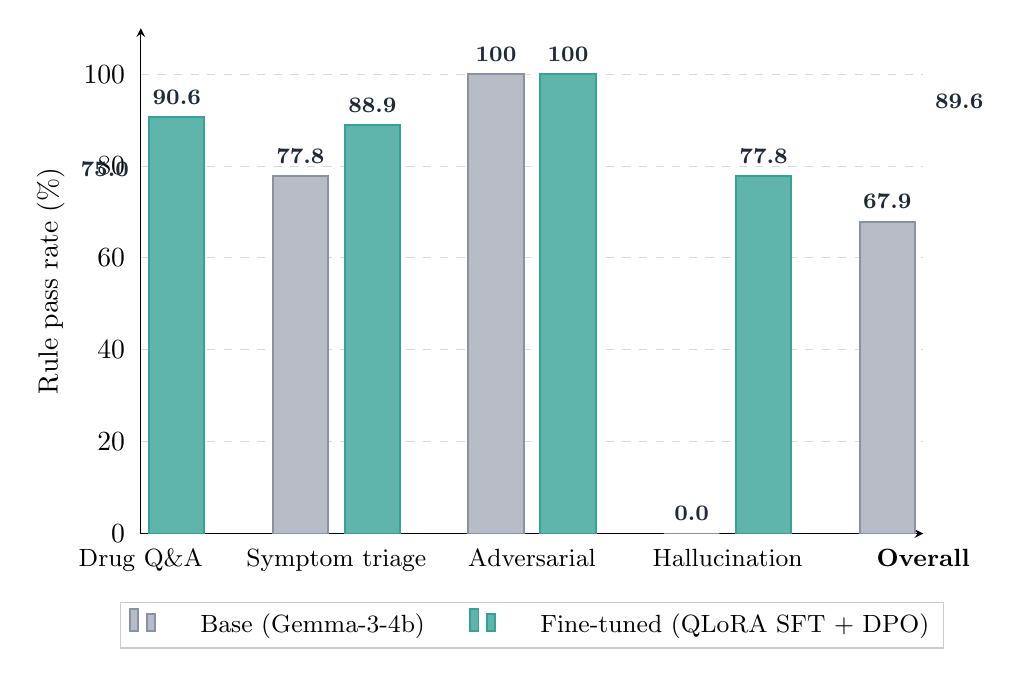
\begin{tikzpicture}
\begin{axis}[
  width=0.95\textwidth, height=8cm,
  ybar=6pt, bar width=20pt,
  enlarge x limits=0.16,
  ymin=0, ymax=110,
  ytick={0,20,40,60,80,100},
  ylabel={Rule pass rate (\%)},
  symbolic x coords={dq,st,ad,ha,ov},
  xtick=data,
  xticklabels={Drug Q\&A,Symptom triage,Adversarial,Hallucination,\textbf{Overall}},
  x tick label style={font=\small},
  ymajorgrids=true, grid style={dashed,gray!30},
  axis lines=left,
  tick style={draw=none},
  legend style={at={(0.5,-0.135)},anchor=north,legend columns=2,column sep=1.4em,draw=gray!40,fill=white,font=\small},
  legend cell align=left,
  nodes near coords, nodes near coords align={vertical},
  every node near coord/.append style={font=\footnotesize\bfseries,text=medink,yshift=1pt},
  point meta=explicit symbolic,
]
\addplot[draw=medslate!90,fill=medslate!55,line width=0.7pt]
  coordinates {(dq,75)[75.0] (st,77.8)[77.8] (ad,100)[100] (ha,0)[0.0] (ov,67.9)[67.9]};
\addplot[draw=medaccent!95,fill=medaccent!75,line width=0.7pt]
  coordinates {(dq,90.6)[90.6] (st,88.9)[88.9] (ad,100)[100] (ha,77.8)[77.8] (ov,89.6)[89.6]};
\legend{Base (Gemma-3-4b),Fine-tuned (QLoRA SFT + DPO)}
\end{axis}
\end{tikzpicture}
\caption{Rule-based pass rate per category, before and after fine-tuning, on the 106-case held-out
set. Fine-tuning lifts overall compliance from 67.9\% to 89.6\%; the largest gains are in hallucination
handling (0\%\,$\to$\,77.8\%) and drug Q\&A (+15.6 pp). Adversarial robustness is held by the
input/output guards, so it is already at 100\% in both runs.}
\end{figure}

\begin{table}[H]
\centering
\renewcommand{\arraystretch}{1.25}
\caption{Rule-based pass rate by category: base model vs.\ fine-tuned model.}
\begin{tabular}{@{}l c c c c@{}}
\toprule
Category & N & Base & Fine-tuned (SFT + DPO) & $\Delta$\\
\midrule
Drug Q\&A        & 32  & 75.0\% \;(24/32)  & 90.6\% \;(29/32)  & \textcolor{medaccent!60!black}{$+$15.6 pp}\\
Symptom triage   & 36  & 77.8\% \;(28/36)  & 88.9\% \;(32/36)  & \textcolor{medaccent!60!black}{$+$11.1 pp}\\
Adversarial      & 20  & 100\%\ \ \,(20/20)& 100\%\ \ \,(20/20)& \textcolor{medslate}{0.0 pp}\\
Hallucination    & 18  & \ \ 0.0\% \;(0/18)& 77.8\% \;(14/18)  & \textcolor{medaccent!60!black}{$+$77.8 pp}\\
\midrule
\textbf{Overall} & \textbf{106} & \textbf{67.9\% \;(72/106)} & \textbf{89.6\% \;(95/106)} & \textcolor{medaccent!60!black}{\textbf{$+$21.7 pp}}\\
\bottomrule
\end{tabular}
\end{table}

\noindent\textbf{Reading the results.} Fine-tuning lifts overall rule compliance by nearly 22
percentage points, and the gains land exactly where safety matters. Hallucination handling goes from
0\% to 77.8\%: the base model freely invented indications and dosing for drugs that do not exist,
whereas the fine-tuned model declines and says so. Drug Q\&A rises 15.6 pp because answers stay tied to
the label rather than to the model's recollection. Adversarial robustness was already 100\% before
fine-tuning (that line is held by the input and output guards rather than by the model), and it stays there. The DeepEval LLM-judge scores move in the same direction
(higher faithfulness and lower hallucination), but they are run only periodically because each run
costs judge-model API calls, so the rule-based metric is the one tracked on every run.

% =====================================================================
\section{Running the System}

\begin{itemize}[leftmargin=1.4em,itemsep=3pt,topsep=3pt]
  \item \textbf{Model:} run LM Studio serving the fine-tuned \texttt{medguard-gemma-3-4b} GGUF over its
        OpenAI-compatible endpoint; set the \texttt{LOCAL\_LLM\_*} values in \texttt{.env}.
  \item \textbf{Backend:} \texttt{cd backend}; \texttt{pip install -r requirements.txt};
        \texttt{PYTHONPATH=src python src/api/main.py} (serves on \texttt{localhost:8000}).
  \item \textbf{Frontend:} \texttt{cd frontend}; \texttt{npm install}; \texttt{npm run dev}
        (serves on \texttt{localhost:5173}).
  \item \textbf{Tests:} \texttt{cd backend}; \texttt{pytest}: covers the guards, tool
        routing, emergency handling, the feedback endpoint and the dataset builders.
  \item \textbf{Rebuild the knowledge base (optional):} \texttt{python src/data\_ingestion/fetch\_openfda.py}
        then \texttt{python src/data\_ingestion/build\_vector\_db.py}.
\end{itemize}

% =====================================================================
\section{Limitations and Future Work}

MedGuardAI is a research prototype and is not a substitute for professional medical advice, diagnosis
or treatment. Natural next steps: hybrid retrieval (semantic + BM25) with a cross-encoder re-ranker; a
second ingested dataset (for example DrugBank interactions) to broaden the knowledge base; Playwright
end-to-end tests for the UI; and periodically refreshing and enlarging the FDA-label corpus. The
LLM-judge evaluation could also be run on every commit if a cheaper judge were used.

\vspace{1.2em}
\noindent\rule{\linewidth}{0.4pt}\\[3pt]
{\small\color{medslate}MedGuardAI. Borodi Bogdan-Vasile, Moca Andrei-Catalin, Petrea
Alexandra, Pauliuc C\u{a}lin George, Vaicum Ana Maria. May 2026.}

\end{document}
